\usepackage[english] {babel}
\usepackage[T1]      {fontenc}
\usepackage{hyperref}

\usepackage{amsmath, amsfonts, graphicx}
\usepackage{tikz}
\usepackage{csquotes}
\usepackage{longtable}
\usepackage{colortbl}%
  \newcommand{\myrowcolour}{\rowcolor[gray]{0.925}}


\setbeamersize
  {text margin left=1em, text margin right=1em}

\title
  [Scoring an SDO]
  {Scoring a Software Development Organization\\ with a Single Number}

\author
  {Ryan M. Swanstrom}

\date
  {April 6, 2015}

\institute[SDSU]
  {South Dakota State University}

\begin{document}

\maketitle

\subsection{About Ryan}
\begin{frame}
  {Ryan M. Swanstrom}
  
  \begin{enumerate}
    \item Professional Software Engineer
    \item Blogger/Data Scientist
    \begin{enumerate}
        \item \href{http://101.datascience.community}{Data Science 101 Blog}
        \item Guest Blogger for \href{http://www.datakind.org/blog/}{DataKind}
    \end{enumerate}
    \item Many Other Things
    \item Started this PhD thing in 2006
  \end{enumerate}
\end{frame}


\subsection{TOC}
\begin{frame}{Overview}

  \tableofcontents

\end{frame}

\section{Overview and Background}

    \subsection{Software Development Organization}
    
        \begin{frame}{Software Development Organization (SDO)?}
            \begin{displayquote}
                 A \textbf{Software Development Organization (SDO)} is any
                 organization or subset of an organization that is 
                 responsible for the creation, deployment, and 
                 maintenance of software. 
            \end{displayquote}
        \end{frame}
        
    \subsection{Software Engineering}
        \begin{frame}{Software Engineering?}
            \begin{displayquote}
                 \textbf{Software} is not just the
                    programs but also all associated documentation and 
                    configuration data which is
                    needed to make these programs operate correctly
                    \cite{Sommerville2001}
            \end{displayquote} 
            
            \begin{displayquote}
                \textbf{Software Engineering} is the application 
                of a systematic, disciplined, quantifiable
                approach to the development, operation, and maintenance of software
                \cite{Ieee1990} 
            \end{displayquote} 
        \end{frame}
    
    \subsection[SDLC]{Software Development Life Cycle}
        \begin{frame}{Software Development Life Cycle (SDLC)?}
            \begin{figure}[ht]
                \centering
                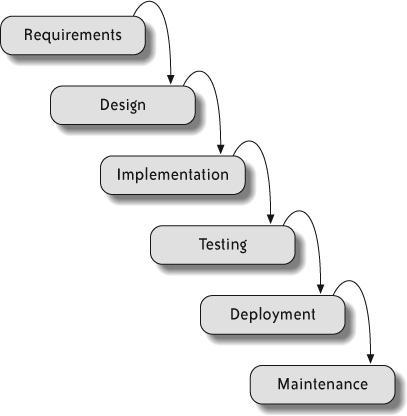
\includegraphics[scale=.86]{images/waterfall.png}
                \caption{SDLC, adapted from \cite{Hibbs2009} }
            \end{figure}
        \end{frame}
    
    \subsection{The Problem}
        \begin{frame}{What is Wrong?}
            \begin{itemize}
                \item Performance is difficult to measure
                \item Inconsistent
                \item Complicated
                \item Overwhelming
            \end{itemize}
        \end{frame}
    
\section{CRI}

    \subsection{CRI Overview}
        \begin{frame}{What is CRI?}
            \begin{displayquote}
                The \textit{Cumulative Result Indicator (CRI)} is an algorithm to provide a single 
                number score to measure the performance of an SDO. 
            \end{displayquote}
            \begin{enumerate}
                \item Quality
                \item Availability
                \item Satisfaction
                \item Schedule
                \item Requirements
            \end{enumerate}
        \end{frame} 
        
        \begin{frame}{CRI Attributes}
            \begin{itemize}
                \item The range of scores must have equal values above and below 0
                \item The minimum score must equate to the worst possible 
                    performance, however that is defined
                \item Similarly, the maximum score must equate to the best possible performance.  
                \item A score of 0 must be average (or expected) performance
                \item All individual elements must have the same scoring range
            \end{itemize}
        \end{frame} 
        
    \subsection{Quality}
        \begin{frame}{Quality Data}
            \centering
            \begin{tabular}{l | r | r}
                 {\bfseries Column Name}
                 & {\bfseries Data Type}
                 &  \\
                
                Application ID & String (factor) & Required \\
                \myrowcolour%
                Frequency Date & Date & Required \\
                Development Effort & Integer & Required \\
                \myrowcolour%
                Testing Effort & Integer & Optional \\ 
                SIT Defects & Integer & Optional \\ 
                \myrowcolour%
                UAT Defects & Integer  & Optional \\ 
                PROD Defects & Integer  & Required \\
                
            \end{tabular}
        \end{frame} 
        \begin{frame}{Quality Formula}
            \begin{displaymath}
               S_{1_i} = \left\{
                 \begin{array}{lr}
                   \text{where } f_i \geq d_i & :  \frac{f_i - d_i}{f_i} \times k  \\
                   \text{where } d_i > f_i  & : \frac{f_i-d_i }{\sigma_i^2} \times k
                 \end{array}
               \right] 
            \end{displaymath} 
            
            \begin{itemize}
                \item $S_{1_i}$ is the quality score for Application ID $i$
                \item $k$ scaling factor to produce results in the range $[-k,k]$
                \item $d_i$ is the actual PROD defects for Application ID $i$
                \item $f_i$ is the function to predict PROD defects for Application $i$ based upon 
                    \textit{UAT Defects}, \textit{SIT Defects}, \textit{Testing Effort}, 
                    and \textit{Development Effort}
                \item $\sigma_i^2$ is the estimated variance for Application $i$
            \end{itemize}
        \end{frame} 
    \subsection{Availability}
        \begin{frame}{Availability Data}
            \centering
            \begin{tabular}{l | r | r}
            {\bfseries Column Name}
                 & {\bfseries Data Type}
                 &  \\
                
                Service ID & String  & Required \\
                \myrowcolour%
                Frequency Date & Date & Required \\
                Uptime & Float & Optional \\
                \myrowcolour%
                Scheduled Downtime & Float & Optional \\
                Unscheduled Downtime & Float  & Optional \\
                \myrowcolour%
                Percent Uptime & Float & Required \\
                Expected Percent Uptime & Float & Required \\
            \end{tabular}
        \end{frame} 
        \begin{frame}{Availability Formula }
            \begin{displaymath}
               S_{2_i} = \left\{
                 \begin{array}{lr}
                   \text{where } A_{a_i} \leq A_{e_i} & : \left[ \frac{A_{a_i} - A_{e_i}}{A_{e_i}}\times k \right] \\
                   \text{where } A_{a_i} > A_{e_i}  & : \left[ \frac{A_{a_i} - A_{e_i} }{1-A_{e_i}}\times k \right]
                 \end{array}
               \right. 
            \end{displaymath}
            
            \begin{itemize}
                \item $S_{2_i}$ is the availability score for System ID $i$
                \item $k$ scaling factor to produce results in the range $[-k,k]$
                \item $A_{a_i}$ actual availability for System ID $i$
                \item $A_{e_i}$ expected availability for System ID $i$
            \end{itemize}
        \end{frame} 
    \subsection{Satisfaction}
        \begin{frame}{Satisfaction Data}
            \centering
            \begin{tabular}{l | r | r}
                {\bfseries Column Name}
                 & {\bfseries Data Type}
                 &  \\
                
                Question ID & String  & Required \\
                \myrowcolour%
                Question Text & String  & Optional \\
                Respondent ID & String & Optional \\
                \myrowcolour%
                Frequency Date & Date & Required \\
                Response & Integer & Required \\
                \myrowcolour%
                Response Date & Date & Optional \\
                Application ID & String & Optional \\
            \end{tabular}
        \end{frame} 
        \begin{frame}{Satisfaction Formula }
            \[
                S_{3_i} =  \frac{2}{max-min}k \cdot \frac{ \sum^m_{j=1}(a_{ij}-\frac{min + max}{2})}{m} = k \cdot \frac{ \sum^m_{j=1}(\frac{2a_{ij}-min-max}{max-min})}{m}
            \]
            
            \begin{itemize}
                \item $S_{3_i}$ is the satisfaction score for Question ID $i$
                \item $k$ scaling factor to produce results in the range $[-k,k]$
                \item $a_{ij}$ answer to question $i$ for respondent $j$
                \item $m$ number of respondents
                \item $min$ minimum score for a question
                \item $max$ maximum score for a question
            \end{itemize}
        \end{frame} 
    \subsection{Schedule}
        \begin{frame}{Schedule Data}
            \centering
            \begin{tabular}{l | r | r}
                {\bfseries Column Name}
                 & {\bfseries Data Type}
                 &  \\
                
                Project ID & String  & Required \\
                \myrowcolour%
                Frequency Date & Date & Required \\
                Scheduled Start Date & Date & Required \\
                \myrowcolour%
                Scheduled Finish Date & Date & Required \\
                Actual Start Date & Date  & Optional \\
                \myrowcolour%
                Actual Finish Date & Date  & Required \\
            \end{tabular}
        \end{frame} 
        \begin{frame}{Schedule Formula }
            \begin{equation}
                S_{4_i} = 2k \cdot \left(CDF(\Delta_i) - \frac{1}{2} \right)
            \end{equation}
            where
            \begin{itemize}
                \item $S_{4_i}$ is the schedule score for Project ID $i$
                \item $\Delta_i$ is the proportion the schedule was missed for Project ID $i$
                \item $k$ scaling factor to produce results in the range $[-k,k]$
            \end{itemize}
        \end{frame} 
    \subsection{Requirements}
        \begin{frame}{Requirements Data}
            \centering
            \begin{tabular}{l | r | r}
                {\bfseries Column Name}
                 & {\bfseries Data Type}
                 &  \\
                
                Project ID & String  & Required \\
                \myrowcolour%
                Frequency Date & Date & Required \\
                Scheduled Requirements & Integer & Required \\
                \myrowcolour%
                Actual Requirements & Integer  & Required \\
            \end{tabular}
        \end{frame} 
        \begin{frame}{Requirements Formula }
        \begin{displaymath}
            S_{5_i} = \left\{
             \begin{array}{lr}
               \text{where } R_{a_i} > R_{s_i} \cdot (b + 1) & :  1 \cdot k \\
               \text{where } R_{a_i} \leq R_{s_i} & : \left[ \frac{R_{a_i} - R_{s_i}}{R_{s_i}}\cdot k \right] \\
               \text{where } R_{a_i} > R_{s_i}  & : \left[ \frac{R_{a_i} - R_{s_i} }{b \cdot R_{s_i}}\cdot k \right]
             \end{array}
            \right. 
            \end{displaymath}
            
            \begin{itemize}
                \item $S_{5_i}$ is the requirements score for Project ID $i$
                \item $k$ scaling factor to produce results in the range $[-k,k]$
                \item $R_{a_i}$ actual requirements completed for Project ID $i$
                \item $R_{s_i}$ expected requirements completed for Project ID $i$
                \item $b$ multiplier to determine the upper bound
            \end{itemize}
        \end{frame} 
    \subsection{Overall}
        \begin{frame}{Overall Formula}
            \[
                CRI =\sum\limits^n_{i=1} w_i S_i 
                    \text{ where } \sum\limits^n_{i=1} w_i = 1
            \]
            
            \begin{itemize}
                \item $CRI$ is the overall CRI score for the time frequency
            \end{itemize}
        \end{frame} 

    \subsection{Storage Framework}
        \begin{frame}{SDLC-AE}
            \begin{figure}[ht]
                \centering
                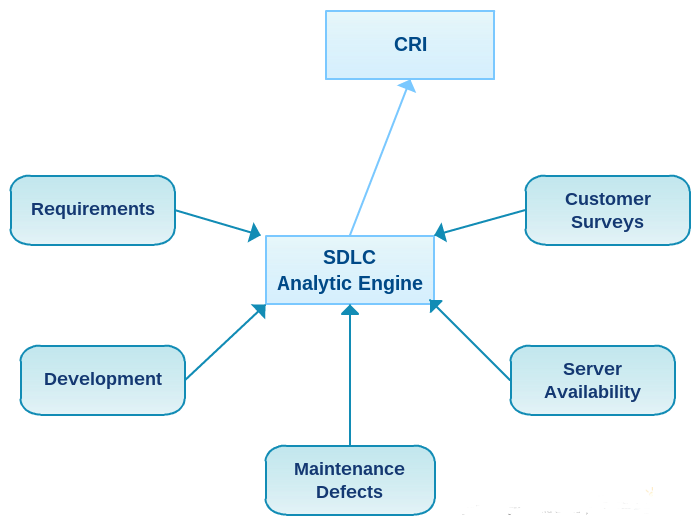
\includegraphics[scale=.5]{images/sdlcae.png}
            \end{figure}
        \end{frame}

\section{Case Study}
        \begin{frame}{Case Study Overview}
            \begin{itemize}
                \item SDO of a Large Financial Institution
                \item Data spans years 2007 - 2015
                \item $k = 100$
                \item Equal Weighting
                \item 4 Elements (Quality, Availability, Schedule, Requirements)
            \end{itemize}
        \end{frame}
    \subsection{Quality}
        \begin{frame}{CRI Quality Scores}
            \begin{figure}
                \centering
                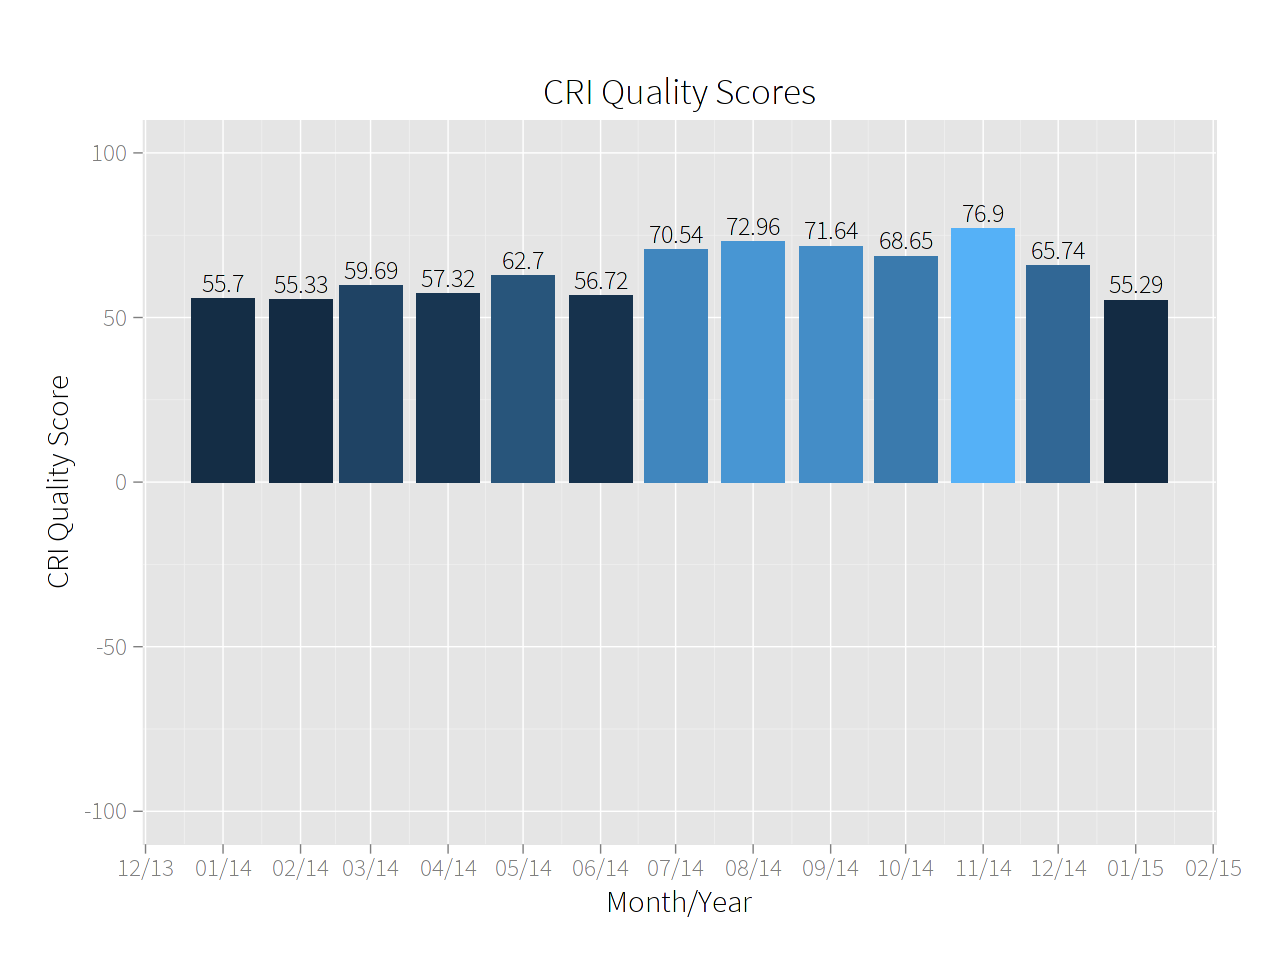
\includegraphics[scale=.23]{images/quality_scores.png}
            \end{figure}
        \end{frame}
    \subsection{Availability}
        \begin{frame}{CRI Availability Scores}
            \begin{figure}
                \centering
                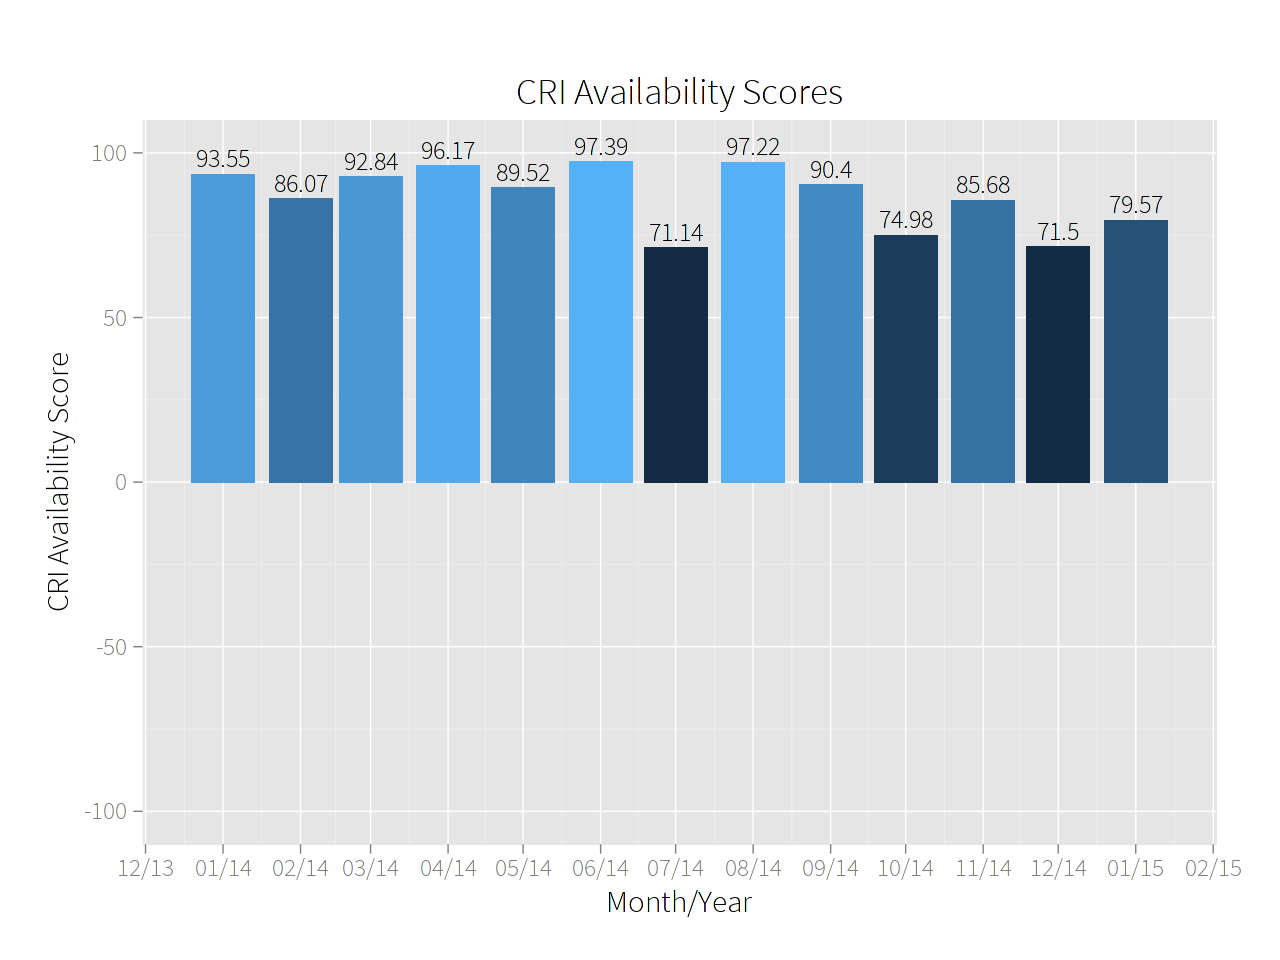
\includegraphics[scale=.23]{images/availability_scores.png}
            \end{figure}
        \end{frame}
    \subsection{Schedule}
        \begin{frame}{CRI Schedule Scores}
            \begin{figure}
                \centering
                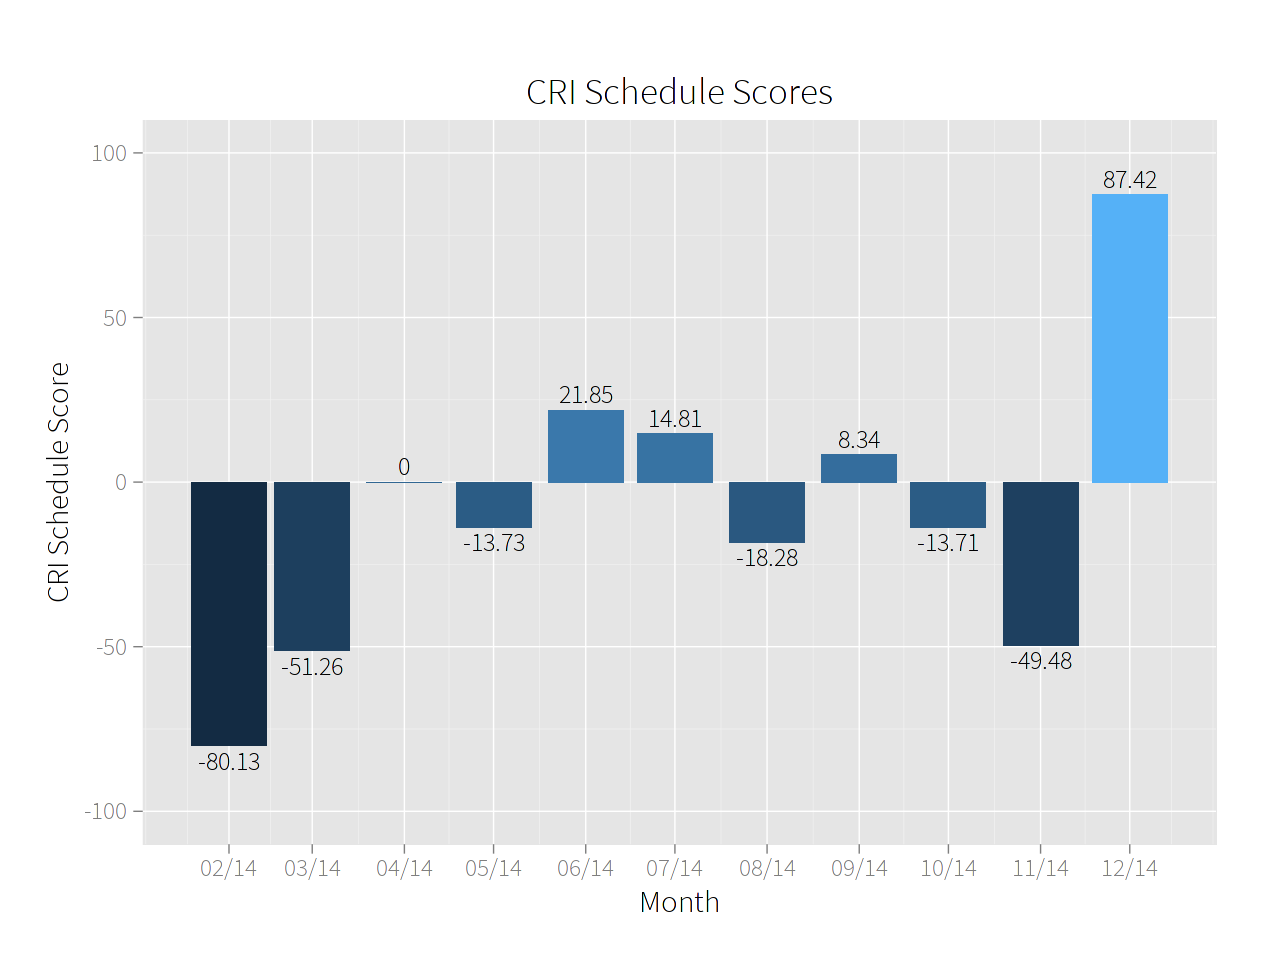
\includegraphics[scale=.23]{images/schedule_scores.png}
            \end{figure}
        \end{frame}
    \subsection{Requirements}
        \begin{frame}{CRI Requirements Scores}
            \begin{figure}
                \centering
                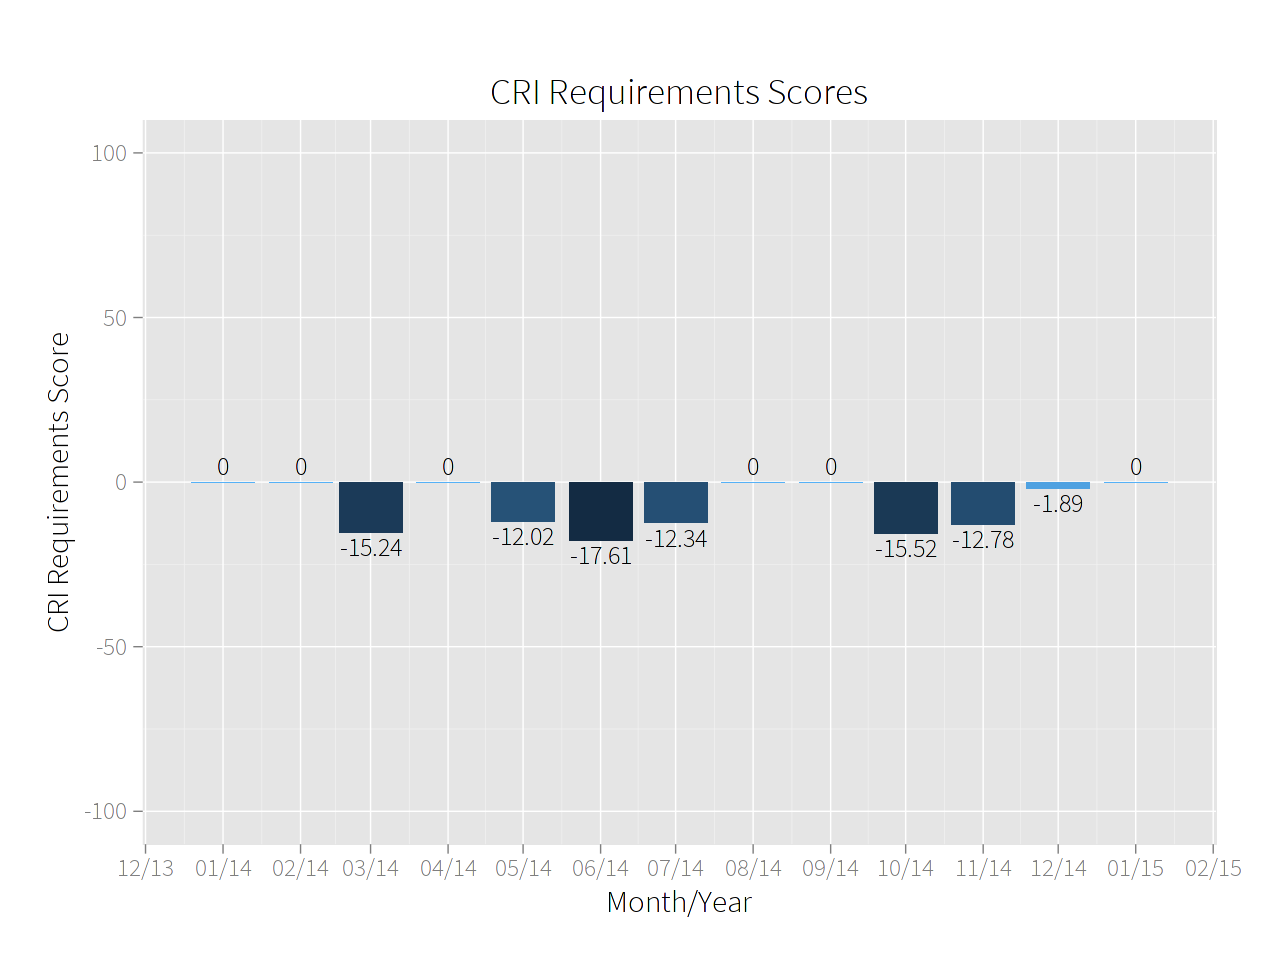
\includegraphics[scale=.23]{images/requirements_scores.png}
            \end{figure}
        \end{frame}
    \subsection{Overall}
        \begin{frame}{CRI Scores}
            \begin{figure}
                \centering
                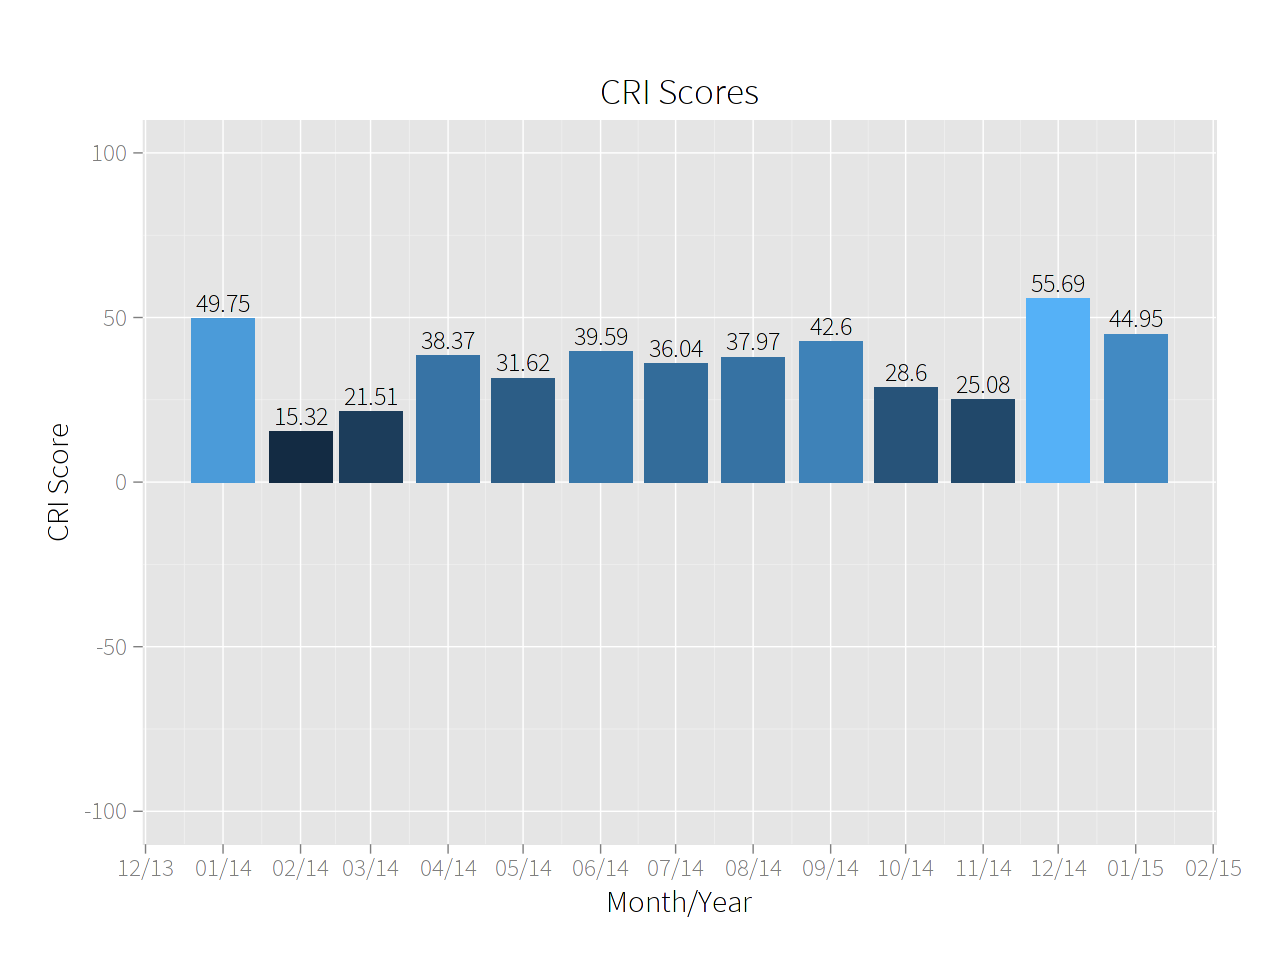
\includegraphics[scale=.23]{images/cri_scores.png}
            \end{figure}
        \end{frame}

\section{Conclusion}

    \subsection{Questions}
        \begin{frame}{Feedback}
            \center 
            Thanks for attending
            
            Questions / Thoughts
          
        \end{frame}

    \subsection{References}
        \begin{frame}{References}
            \bibliographystyle{acm}
            \bibliography{references}
          
        \end{frame}

\end{document}
